\documentclass{article}\usepackage[]{graphicx}\usepackage[]{xcolor}
% maxwidth is the original width if it is less than linewidth
% otherwise use linewidth (to make sure the graphics do not exceed the margin)
\makeatletter
\def\maxwidth{ %
  \ifdim\Gin@nat@width>\linewidth
    \linewidth
  \else
    \Gin@nat@width
  \fi
}
\makeatother

\definecolor{fgcolor}{rgb}{0.345, 0.345, 0.345}
\newcommand{\hlnum}[1]{\textcolor[rgb]{0.686,0.059,0.569}{#1}}%
\newcommand{\hlsng}[1]{\textcolor[rgb]{0.192,0.494,0.8}{#1}}%
\newcommand{\hlcom}[1]{\textcolor[rgb]{0.678,0.584,0.686}{\textit{#1}}}%
\newcommand{\hlopt}[1]{\textcolor[rgb]{0,0,0}{#1}}%
\newcommand{\hldef}[1]{\textcolor[rgb]{0.345,0.345,0.345}{#1}}%
\newcommand{\hlkwa}[1]{\textcolor[rgb]{0.161,0.373,0.58}{\textbf{#1}}}%
\newcommand{\hlkwb}[1]{\textcolor[rgb]{0.69,0.353,0.396}{#1}}%
\newcommand{\hlkwc}[1]{\textcolor[rgb]{0.333,0.667,0.333}{#1}}%
\newcommand{\hlkwd}[1]{\textcolor[rgb]{0.737,0.353,0.396}{\textbf{#1}}}%
\let\hlipl\hlkwb

\usepackage{framed}
\makeatletter
\newenvironment{kframe}{%
 \def\at@end@of@kframe{}%
 \ifinner\ifhmode%
  \def\at@end@of@kframe{\end{minipage}}%
  \begin{minipage}{\columnwidth}%
 \fi\fi%
 \def\FrameCommand##1{\hskip\@totalleftmargin \hskip-\fboxsep
 \colorbox{shadecolor}{##1}\hskip-\fboxsep
     % There is no \\@totalrightmargin, so:
     \hskip-\linewidth \hskip-\@totalleftmargin \hskip\columnwidth}%
 \MakeFramed {\advance\hsize-\width
   \@totalleftmargin\z@ \linewidth\hsize
   \@setminipage}}%
 {\par\unskip\endMakeFramed%
 \at@end@of@kframe}
\makeatother

\definecolor{shadecolor}{rgb}{.97, .97, .97}
\definecolor{messagecolor}{rgb}{0, 0, 0}
\definecolor{warningcolor}{rgb}{1, 0, 1}
\definecolor{errorcolor}{rgb}{1, 0, 0}
\newenvironment{knitrout}{}{} % an empty environment to be redefined in TeX

\usepackage{alltt}
\usepackage{bm}
\usepackage{amsmath} %This allows me to use the align functionality.
                     %If you find yourself trying to replicate
                     %something you found online, ensure you're
                     %loading the necessary packages!
\usepackage{amsfonts}%Math font
\usepackage{graphicx}%For including graphics
\usepackage{hyperref}%For Hyperlinks
\usepackage[shortlabels]{enumitem}% For enumerated lists with labels specified
                                  % We had to run tlmgr_install("enumitem") in R
\hypersetup{colorlinks = true,citecolor=black} %set citations to have black (not green) color
\usepackage{natbib}        %For the bibliography
\setlength{\bibsep}{0pt plus 0.3ex}
\bibliographystyle{apalike}%For the bibliography
\usepackage[margin=0.50in]{geometry}
\usepackage{float}
\usepackage{multicol}

%fix for figures
\usepackage{caption}
\newenvironment{Figure}
  {\par\medskip\noindent\minipage{\linewidth}}
  {\endminipage\par\medskip}
\IfFileExists{upquote.sty}{\usepackage{upquote}}{}
\begin{document}

\vspace{-1in}
\title{Lab 8 -- MATH 240 -- Computational Statistics}

\author{
  Henry Sun \\
  Colgate University  \\
  Department of Mathematics  \\
  {\tt }
}

\date{04/01/2025}

\maketitle

\begin{multicols}{2}\raggedcolumns
\begin{abstract}
In this lab, we explored the beta distribution in great detail. We discussed probability functions, parameters, and properties of the beta distribution. We then use two point techniques, the method of moments (MOM) and the maximum likelihood (MLE) to help us model country death rates. Overall, we found that the estimated parameters from MLE we more accurate than MOM compared to actual parameters suggested. 
\end{abstract}

\noindent \textbf{Keywords:} Point estimation; continuous probability distributions; parameters

\section{Introduction}
The beta distribution is a continuous distribution used to model a random variable $X$ ranging from $0$ to $1$ (the distribution's support), making it particularly useful for modeling proportions, probabilities, and rates. For some data, like the example we will look at later in the lab, data must be transformed to fit the support. The beta distribution is remarkably flexible in its shape; it can be right-skewed, left-skewed, or symmetric. \\
\indent Section $2$ provides a more in-depth overview of the beta distribution, including the Probability Density Function, support, and parameters. Section $3$ discusses the properties of the beta distribution using four specific cases. Sections $4$ and $5$ contextualize point estimators (Method of Moments and Maximum Likelihood) and explores the beta distribution further with an example of real-life data. 

\section{Density Functions and Parameters}
As the beta distribution is a continuous distribution, it has a probability density function (PDF) and a cumulative density function (CDF). It takes two shape parameters, $\alpha$ and $\beta$, which are both positive numbers. In \texttt{R}, the parameters for $\alpha$ and $\beta$ are \texttt{shape1} and \texttt{shape2}. The beta distribution's probability density function is given as:
 \[f_X(x|\alpha, \beta) = \frac{\Gamma(\alpha + \beta)}{\Gamma\alpha\Gamma\beta} x^{\alpha-1}(1-x)^{\beta-1}I(x \in [0,1]).\]
\indent For the beta distribution, $I(x \in [0,1]) = 1$ when $x \in [0,1]$ and $0$ otherwise, as the support of a random variable $X$ is $[0,1]$ in the beta distribution. 

\section{Properties and Statistics}
Various properties of the beta distribution are based on the shape parameters of the beta distribution. The beta distribution is very flexible with regards to its shape. The various statistics, such as the mean, variance, skewness, and excess kurtosis can be written in terms of $\alpha$ and $\beta$: 
 \begin{align*}
 E(X) = \frac{\alpha}{\alpha + \beta} \tag{The Mean}\\
var(X) = \frac{\alpha\beta}{(\alpha + \beta)^2(\alpha + \beta + 1)} \tag{The Variance} \\
skew(X) = \frac{2(\beta - \alpha)\sqrt{\alpha + \beta + 1}}{(\alpha + \beta + 2)\sqrt{\alpha\beta}} \tag{The Skewness}
 \end{align*}
 \[kurt(X) = \frac{6[(\alpha - \beta)^2(\alpha + \beta + 1) - \alpha\beta(\alpha + \beta + 2)]}{\alpha\beta(\alpha + \beta + 2)(\alpha + \beta + 3)}\]
\begin{flushright}
(The Excess Kurtosis)
\end{flushright}

\indent It's key to note that in \texttt{R}, \verb|kurt()| calculates the excess kurtosis and not the kurtosis. Instead, kurtosis = excess kurtosis + 3, or \verb|kurt(X) + 3|. \\
\indent However, by computing the moments of the beta function, we write each statistic as a combination of various $k$th centered and uncentered moments. 
\begin{align*}
 \mu_X = E(X) \tag{The Mean}\\
 var(X) = \sigma^2_X = E[(X-\mu_X)]^2 \tag{The Variance}\\
 skew(X) = \frac{E[(X - \mu_X)^3]}{E[(X-\mu_X)^2]^{3/2}} \tag{The Skewness}\\
 kurt(X) = \frac{E[(X-\mu_X)^4]}{E[(X-\mu_X)^2]^2} - 3 \tag{The Excess Kurtsosis}
\end{align*}
\indent For the beta distribution, the $k$th uncentered and centered moments are
\[E(X^{k}) = \int_{\chi}^{} x^{k}f_x(x) \,dx \]
\begin{center}
and 
\end{center}
\[E((X-\mu_X)^{k}) = \int_{\chi}^{} (x-\mu_X)^{k}f_x(x) \,dx \]
respectively. For the purposes of this lab, we wrote a function \verb|beta.moment(alpha, beta, k, centered)| to help us compute the population-level characteristics using this moments. \\

\indent Due to the beta distribution's flexibility, it can take on numerous different shapes. Below is a table (\autoref{table1}) showing various different summary statistics for four different cases of the beta distribution. Additionally, the actual shape of these different cases can be found in the appendix (\autoref{plot1}). 

\begin{Figure}
\centering
\begin{tabular}{rrrrrrr}
  \hline
  alpha & beta & mean & variance & skewness & e.kurtosis \\ 
  \hline
  2.00 & 5.00 & 0.29 & 0.03 & 0.60 & -0.12 \\ 
  5.00 & 5.00 & 0.50 & 0.02 & 0.00 & -0.46 \\ 
  5.00 & 2.00 & 0.71 & 0.03 & -0.60 & -0.12 \\ 
  0.50 & 0.50 & 0.50 & 0.12 & 0.00 & -1.50 \\ 
   \hline
\end{tabular}
\captionof{table}{Table showing various summary statistics for different shape parameters, $\alpha$ and $\beta$. Notice the large variation in the summary statistics for different shape parameters. \texttt{e.kurtosis} means excess kurtosis.}
\label{table1}
\end{Figure}

\indent As with many other distributions, as the sample size (samples were generated from each known beta distribution) increases, summary statistics calculated on each sample converges towards the true population-level characteristics. A plot of samples (\autoref{plot3}) generated from sizes $0$ to $500$ from the beta($\alpha = 2$, $\beta = 5$) distribution show this property. The cumulative statistics \citep{cumstats} of samples were chaotic in smaller sample sizes, but stabilized at sample size was increased.\\ 
\indent The sampling distributions for summary statistics from the original beta distribution also show an approximately Gaussian distribution (\autoref{plot4}), with the mean of the sampling distributions being approximately the population-level summary statistics.

\section{Estimators}
In class, we discussed two point estimators that help us find the approximate estimates for unknown parameters, $\theta$ in various distributions, the Method of Moments (MOM) and Maximum Likelihood (MLE). In the beta distribution, $\theta$ are the shape parameters $\alpha$ and $\beta$. \\
\indent In many cases, the distribution a set of data follows is unknown, and point estimators can help us come up with a good approximation of the parameters for a distribution that fits the data. \\
\indent The Method of Moments works by equating the first $k$ uncentered population moments with the first $k$ sample moments (assuming that the sample size is large enough where they are approximately equal), setting up an approximate systems of equation to solve for each parameter. In \texttt{R}, we accomplished this by using the \verb|nleqslv()| \citep{nleqslv} to obtain $\alpha$ and $\beta$. For the beta distribution, the first two uncentered population moments are: 
\[E(X) = \frac{\alpha}{\alpha + \beta}\]
\[E(X^2) = \frac{(\alpha + 1)\alpha}{(\alpha + \beta + 1)(\alpha + \beta)}\]
\indent Maximum Likelihood works by first defining the likelihood function: 
\[L(\bm{\theta} | \mathbf{x}) = \prod_{i=1}^{n} f_X(x_i | \bm{\theta})\]
The likelihood function is asking the question: What is the likelihood of observing $\mathbf{x}$? However, in most situations, it is more practical and useful to work with the log likelihood function. For Maximum Likelihood, we are essentially trying to find which parameters maximize the probability of observing $\mathbf{x}$. This basically becomes an optimization problem that can be solved with calculus. In \texttt{R}, this is accomplished by using the \verb|optim()| function. \\
\indent We will apply both MOM and MLE in the Example section, using actual data. 

\section{Example: World Death Rates}
\cite{labdata} suggests that country death rates worldwide can be modeled with a beta distribution, specifically with $\alpha = 8$ and $\beta = 950$. Both MOM and MLE will provide us with slightly different parameters, so we must analyze bias, precision, and mean squared error (MSE) in order to determine which one gives us a closer estimate to the actual parameters. The data also had to be modified, changing the death rate so it would fit the support of the beta distribution.
\[bias = E(\hat{\theta}) - \theta\]
\[precision = \frac{1}{var(\hat{\theta})}\]
\[MSE = var(\hat{\theta}) + (E(\hat{\theta}) - \theta)^2\]

\indent The summaries of these calculations for each method and shape parameter can be found in the table below (\autoref{table3}). Overall, it appears that MLE seems to be the better estimator for this data than MOM. The bias and MSE for the MLE parameters is smaller than MOM, and the precision is higher. However, it's still quite hard to notice the difference between the actual PDF, MLE PDF, and MOM PDF, as shown in \autoref{plot6}. Still, the MLE PDF seems to be marginally better fit for the data. 

\begin{Figure}
\centering
\begin{tabular}{rllrrr}
  \hline
 parameters & method & bias & precision & mse \\ 
  \hline
    Alpha & MOM & 0.08 & 1.83 & 0.63 \\ 
    Alpha & MLE & 0.07 & 2.13 & 0.54 \\ 
    Beta & MOM & 10.29 & 0.00 & 8192.93 \\ 
    Beta & MLE & 9.11 & 0.00 & 7058.82 \\ 
   \hline
\end{tabular}
\captionof{table}{The bias, precision, and MSE for $\alpha$ and $\beta$ with MOM and MLE. Due to the exceedingly small values for $\beta$ precision, it appears as $0$ on the table.}
\label{table3}
\end{Figure}
\indent Just like how the sampling distribution for the summary statistics is approximately Gaussian, the sampling distribution of the shape parameters ,$\alpha$ and $\beta$, follow an approximately Gaussian distribution (\autoref{plot5}), with the actual parameter (shown as a red vertical line), regardless if we are using MOM and MLE. Samples were generated from the actual parameters for the beta distribution fitting the death rates, $\alpha = 8$ and $\beta = 950$. Both estimations are not exact, but can be considered close enough. 

%%%%%%%%%%%%%%%%%%%%%%%%%%%%%%%%%%%%%%%%%%%%%%%%%%%%%%%%%%%%%%%%%%%%%%%%%%%%%%%%
% Bibliography
%%%%%%%%%%%%%%%%%%%%%%%%%%%%%%%%%%%%%%%%%%%%%%%%%%%%%%%%%%%%%%%%%%%%%%%%%%%%%%%%
\vspace{2em}

\begin{tiny}
\bibliography{bib}
\end{tiny}
\end{multicols}

%%%%%%%%%%%%%%%%%%%%%%%%%%%%%%%%%%%%%%%%%%%%%%%%%%%%%%%%%%%%%%%%%%%%%%%%%%%%%%%%
% Appendix
%%%%%%%%%%%%%%%%%%%%%%%%%%%%%%%%%%%%%%%%%%%%%%%%%%%%%%%%%%%%%%%%%%%%%%%%%%%%%%%%
\newpage
\onecolumn
\section{Appendix}
 \begin{figure}[H]
 \begin{center}
\begin{knitrout}
\definecolor{shadecolor}{rgb}{0.969, 0.969, 0.969}\color{fgcolor}
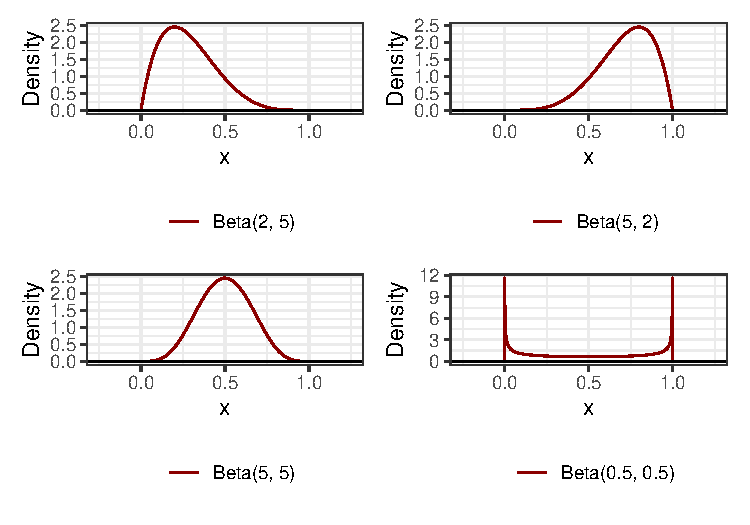
\includegraphics[width=\maxwidth]{figure/unnamed-chunk-2-1} 
\end{knitrout}
 \caption{Plotting of various different beta PDFs.}
 \label{plot1} %we can now reference plot1
 \end{center}
 \end{figure}

\begin{figure}[H]
 \begin{center}
\begin{knitrout}
\definecolor{shadecolor}{rgb}{0.969, 0.969, 0.969}\color{fgcolor}
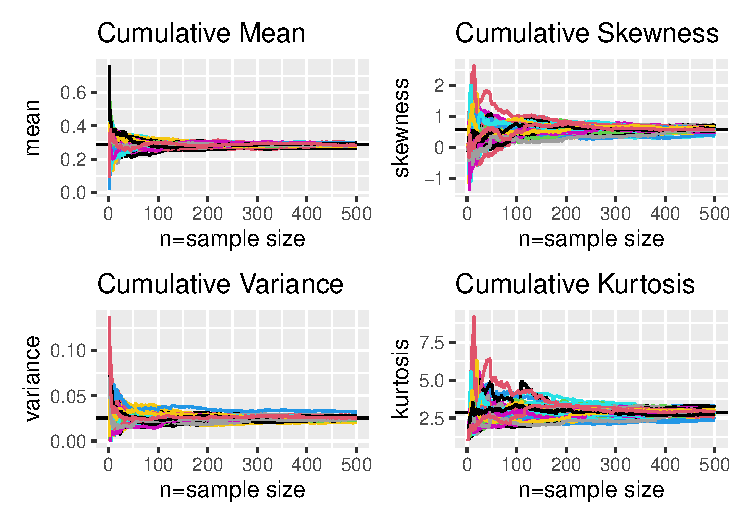
\includegraphics[width=\maxwidth]{figure/unnamed-chunk-3-1} 
\end{knitrout}
 \caption{Plots showing the cumulative statistics, showing how statistics change as sample size increases from $0$ to $500$.}
 \label{plot3} %we can now reference plot1
 \end{center}
 \end{figure}

\begin{figure}[H]
 \begin{center}
\begin{knitrout}
\definecolor{shadecolor}{rgb}{0.969, 0.969, 0.969}\color{fgcolor}
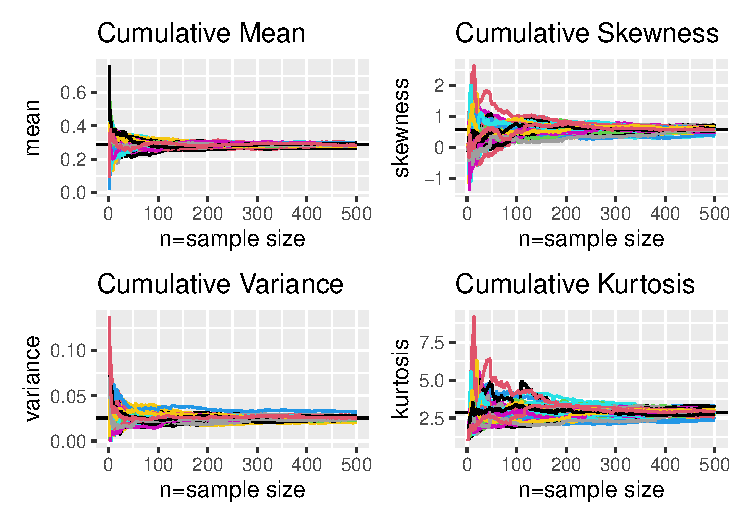
\includegraphics[width=\maxwidth]{figure/unnamed-chunk-4-1} 
\end{knitrout}
 \caption{Sampling Distributions for various summary statistics. The samples were generated from the beta($\alpha = 2$, $\beta = 5$) distribution.}
 \label{plot4} %we can now reference plot1
 \end{center}
 \end{figure}
 

\begin{figure}[H]
 \begin{center}
\begin{knitrout}
\definecolor{shadecolor}{rgb}{0.969, 0.969, 0.969}\color{fgcolor}
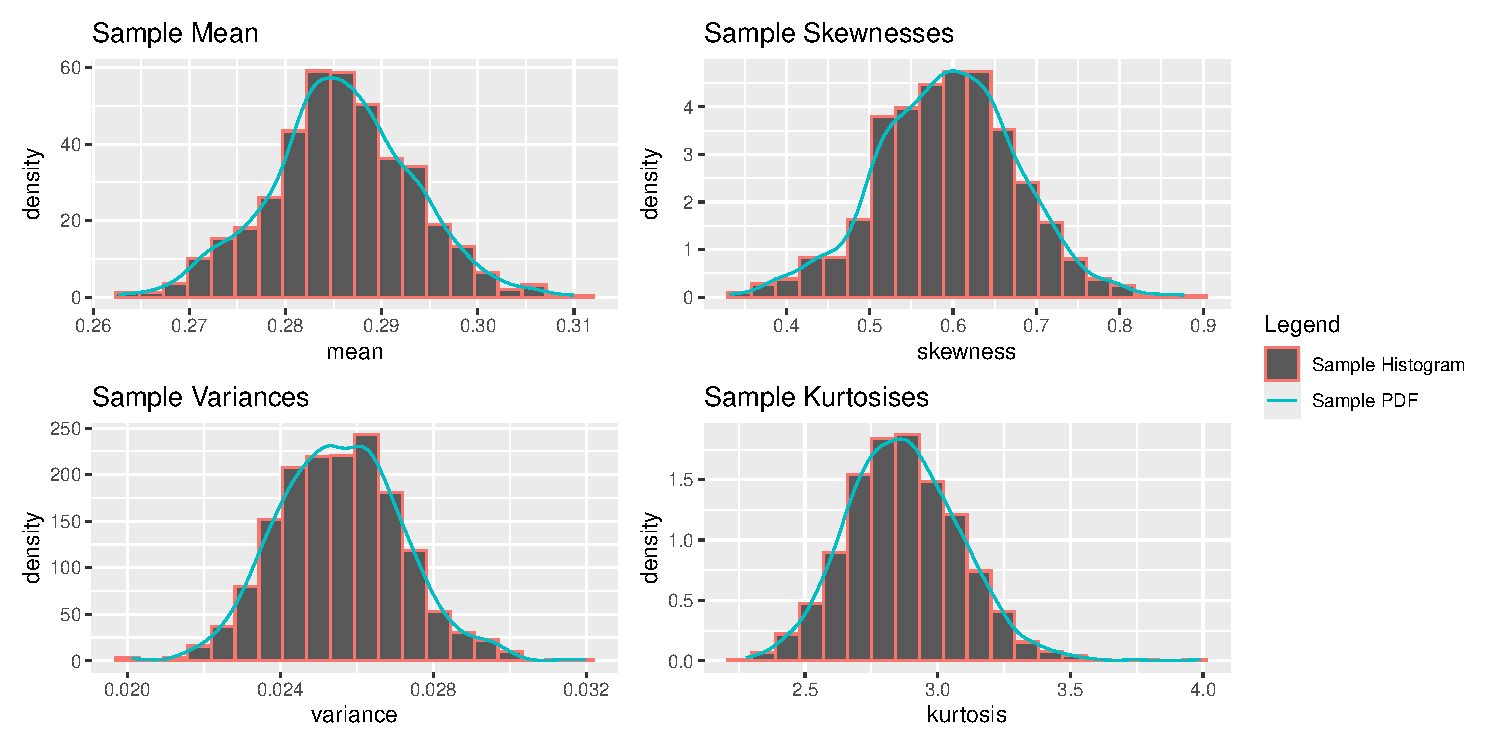
\includegraphics[width=\maxwidth]{figure/unnamed-chunk-5-1} 
\end{knitrout}
 \caption{Sampling Distributions of the shape parmeters $\alpha$ and $\beta$, with resamples generated from the beta($\alpha = 8$, $\beta = 950$) distribution.}
 \label{plot5} %we can now reference plot1
 \end{center}
 \end{figure}

\begin{figure}[H]
 \begin{center}
\begin{knitrout}
\definecolor{shadecolor}{rgb}{0.969, 0.969, 0.969}\color{fgcolor}
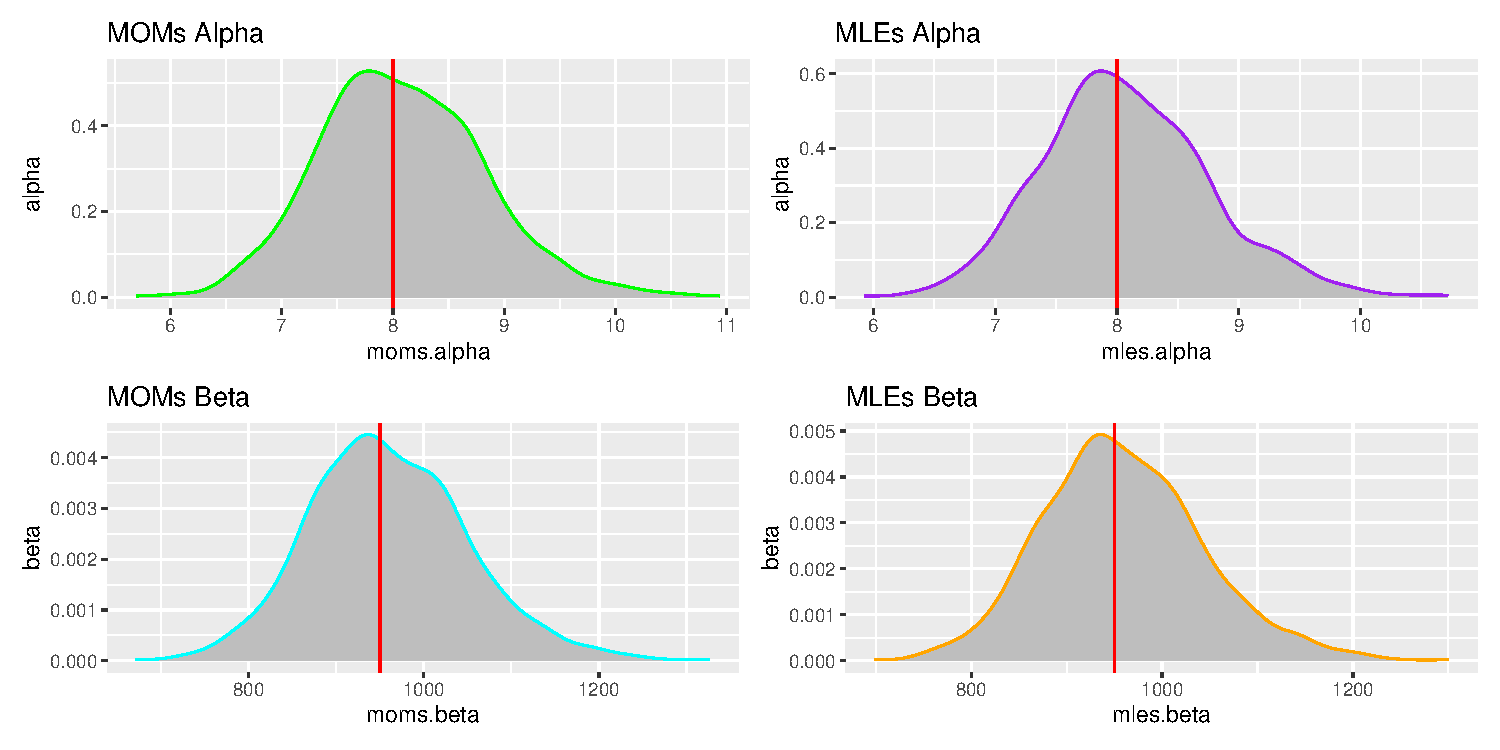
\includegraphics[width=\maxwidth]{figure/unnamed-chunk-6-1} 
\end{knitrout}
 \caption{Death Rates data plotted alongside the actual PDF proposed, and the PDFs from the estimated shape parameters obtained from MOM and MLE. The vertical shows the actual proposed shape parameters.}
 \label{plot6} %we can now reference plot1
 \end{center}
 \end{figure}
\end{document}
